\documentclass[12pt, oneside]{article}
\usepackage[letterpaper, margin=1in]{geometry}
\usepackage[english]{babel}
\usepackage[utf8]{inputenc}
\usepackage{amsmath}
\usepackage{amsfonts}
\usepackage{amssymb}
\usepackage{tikz}
\usepackage{tkz-fct}

\usepackage{fancyhdr}
\pagestyle{fancy}
\fancyhf{}
\rhead{\thepage \\Name: \hspace{1.5in}.\\}
\lhead{BECA / Dr. Huson / 11.1 Algebra 2 Regents prep \\* 18 March 2018 \\* \textbf{Classwork: Polynomial functions and graphs}}

\vspace{1cm}

\renewcommand{\headrulewidth}{0pt}

\title{Problem set template}
\author{Chris Huson}
\date{April 2018}

\begin{document}
%\maketitle

\subsubsection*{\\* \textnormal{Graph carefully using pencil}}

\begin{enumerate}
\item The zeros of a quartic polynomial function $f$ are  $-5, 0, 2, \text{ and } 7$. The polynomial has a positive leading coefficient, $a>0$. Sketch a graph of $y = f(x)$ on the grid below.\\*
\begin{center}
    
\begin{tikzpicture}
    \draw[step=0.25in,gray,very thin] (0,0) grid (12.7,12.7);
    \end{tikzpicture}
\end{center}
Write an equation for $f(x)$ in factored form, assuming the leading coefficient is one.\\*[30pt]
Express the function in standard form. Check that the $y$-intercept on your graph is correct.

\newpage


\item Given that the remainder when  $f(x)=3x^3-9x^2+8x-20$ is divided by $x-3$ is 4. What is the value of $f(3)$? \\*[1in]

\item What is the quotient when $3x^2-9x-12$ is divided by $x + 2$?\\*[3in]

\item Algebraically determine the values of $h$ and $k$ to correctly complete the identity stated below.
\[2x^3-3x^2+7x+3=(x-2)(hx^2+x+9)+k\] %\\*[3in]

\newpage


\item Given: $f(x)=x^2+ 3x - 2$ and $g(x)=2x+3$\\*[5pt]
Express $f(x) \times g(x)$ as a polynomial in standard form. \\*[3in]


\item Simplify the expression $\displaystyle \frac{6x^3+9x^2-5x-4}{2x+1}$, where $x \neq -\frac{1}{2}$. 

\newpage

\item Given the function $f(x)=x^3-4x^2-4x-7$. 
\begin{enumerate}
    \item Using the calculator table function, complete the $y$ values.
    \begin{tabular}{r|r}
    x & f(x)\\ 
    \hline 
    $-4$ & \\[5pt]
    $-3$ & \\[5pt]
    $-2$ & \\[5pt]
    $-1$ & \\[5pt]
    $0$ & \\[5pt]
    $1$ & \\[5pt]
    $2$ & \\[5pt]
    $3$ & \\[5pt]
    $4$ & \\[5pt]
    $5$ & \\ 
    \end{tabular}
    \item Graph the function on the grid below.
    \item Using the calculator graph-solve function, find the roots of the function, rounded to the \emph{nearest hundredth}.
\end{enumerate}
\begin{center}
    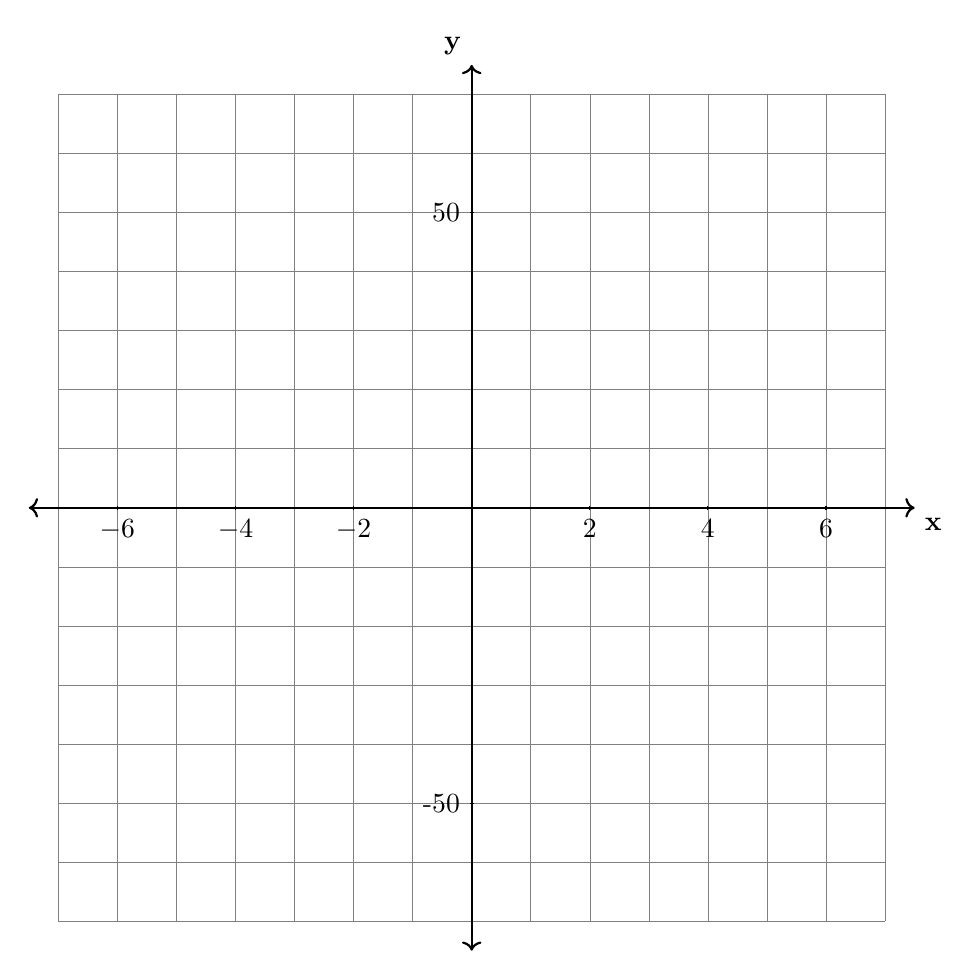
\begin{tikzpicture}[scale=3/4]
    \draw[step=1cm,gray,very thin] (-7,-7) grid (7,7);
    \draw[thick,<->] (-7.5,0) -- (7.5,0) node[anchor=north west] {\textbf{x}};
    \draw[thick,<->] (0,-7.5) -- (0,7.5) node[anchor=south east] {\textbf{y}};
    \foreach \x in {-6, -4, -2, 2, 4, 6} \draw (\x cm,1pt) -- (\x cm,-1pt) node[anchor=north] {$\x$};
    \foreach \y in {5} \draw (1pt,\y cm) -- (-1pt,\y cm) node[anchor=east] {50};
    \foreach \y in {-5} \draw (1pt,\y cm) -- (-1pt,\y cm) node[anchor=east] {-50};    \tkzInit[xmin=-5,xmax=5,ymin=-7,ymax=7,ystep=1]   
%    \tkzFct[color=black,thick,<->,domain = -3.4:7] {0.1*(x*x-4)*(x-5)};
    \end{tikzpicture}
\end{center}

\newpage

\item Sketch a graph with the following characteristics: 
\begin{itemize}
\item three real zeros
\item as $x \rightarrow + \infty$, $f(x) \rightarrow - \infty$
\item as $x \rightarrow - \infty$, $f(x) \rightarrow + \infty$
\end{itemize}
\begin{center}
    \begin{tikzpicture}[scale=2/4]
    \draw[thick,<->] (-7.5,0) -- (7.5,0) node[anchor=north west] {\textbf{x}};
    \draw[thick,<->] (0,-7.5) -- (0,7.5) node[anchor=south east] {\textbf{y}};
    \end{tikzpicture}
\end{center} %Alg2 Regents Jun2016 MC


\item Sketch a graph with the following characteristics: 
\begin{itemize}
\item polynomial function of order four
\item a positive leading coefficient
\item four real zeros
\end{itemize}
\begin{center}
    \begin{tikzpicture}[scale=2/4]
    \draw[thick,<->] (-7.5,0) -- (7.5,0) node[anchor=north west] {\textbf{x}};
    \draw[thick,<->] (0,-7.5) -- (0,7.5) node[anchor=south east] {\textbf{y}};
    \end{tikzpicture}
\end{center}

\newpage

\item For each polynomial graph, state 
\begin{enumerate}
\item its degree,
\item how many distinct zeros it has, and
\item the sign of its leading coefficient.
\end{enumerate}

    \begin{tikzpicture}[scale=2/4]
    %\draw[step=1cm,gray,very thin] (-7,-7) grid (7,7);
    \draw[thick,<->] (-7.5,0) -- (7.5,0) node[anchor=north west] {\textbf{x}};
    \draw[thick,<->] (0,-7.5) -- (0,7.5) node[anchor=south east] {\textbf{y}};
    %\foreach \x in {-6, -4, -2, 2, 4, 6} \draw (\x cm,1pt) -- (\x cm,-1pt) node[anchor=north] {$\x$};
    %\foreach \y in {5} \draw (1pt,\y cm) -- (-1pt,\y cm) node[anchor=east] {50}; %{$\y$};
    \tkzInit[xmin=-6,xmax=6,ymin=-7,ymax=7,ystep=1]   
    \tkzFct[color=black,thick,<->,domain = -4.3:5.2] {-0.1*(x+3)*(x)*(x-4)};
    \end{tikzpicture}
    \begin{tikzpicture}[scale=2/4]
    %\draw[step=1cm,gray,very thin] (-7,-7) grid (7,7);
    \draw[thick,<->] (-7.5,0) -- (7.5,0) node[anchor=north west] {\textbf{x}};
    \draw[thick,<->] (0,-7.5) -- (0,7.5) node[anchor=south east] {\textbf{y}};
    %\foreach \x in {-6, -4, -2, 2, 4, 6} \draw (\x cm,1pt) -- (\x cm,-1pt) node[anchor=north] {$\x$};
    %\foreach \y in {5} \draw (1pt,\y cm) -- (-1pt,\y cm) node[anchor=east] {50}; %{$\y$};
    \tkzInit[xmin=-6,xmax=6,ymin=-7,ymax=7,ystep=1]   
    \tkzFct[color=black,thick,<->,domain = -5.3:4.2] {-0.05*(x+5)*(x+3)*(x-1)*(x-4)};
    \end{tikzpicture}
\\[30pt]
    \begin{tikzpicture}[scale=2/4]
    %\draw[step=1cm,gray,very thin] (-7,-7) grid (7,7);
    \draw[thick,<->] (-7.5,0) -- (7.5,0) node[anchor=north west] {\textbf{x}};
    \draw[thick,<->] (0,-7.5) -- (0,7.5) node[anchor=south east] {\textbf{y}};
    %\foreach \x in {-6, -4, -2, 2, 4, 6} \draw (\x cm,1pt) -- (\x cm,-1pt) node[anchor=north] {$\x$};
    %\foreach \y in {5} \draw (1pt,\y cm) -- (-1pt,\y cm) node[anchor=east] {50}; %{$\y$};
    \tkzInit[xmin=-6,xmax=6,ymin=-7,ymax=7,ystep=1]   
    \tkzFct[color=black,thick,<->,domain = -1.3:5.2] {-0.5*(x-2)*(x-2)};
    \end{tikzpicture}
    \begin{tikzpicture}[scale=2/4]
    %\draw[step=1cm,gray,very thin] (-7,-7) grid (7,7);
    \draw[thick,<->] (-7.5,0) -- (7.5,0) node[anchor=north west] {\textbf{x}};
    \draw[thick,<->] (0,-7.5) -- (0,7.5) node[anchor=south east] {\textbf{y}};
    %\foreach \x in {-6, -4, -2, 2, 4, 6} \draw (\x cm,1pt) -- (\x cm,-1pt) node[anchor=north] {$\x$};
    %\foreach \y in {5} \draw (1pt,\y cm) -- (-1pt,\y cm) node[anchor=east] {50}; %{$\y$};
    \tkzInit[xmin=-6,xmax=6,ymin=-7,ymax=7,ystep=1]   
    \tkzFct[color=black,thick,<->,domain = -3.3:5.2] {0.05*(x*x*x*x-3*x*x*x-9*x*x+10*x+20)};
    \end{tikzpicture}


\newpage

\end{enumerate}
\end{document}